
\section{Introduction}
\label{sec:introduction}
Universal medical imaging models trained on large-scale, diverse datasets represent a significant step toward clinical AI deployment, exhibiting strong generalization across clinical centers and medical tasks~\cite{liu2023clip, butoi2023universeg, yang2024brainmass}.


Initially introduced in natural language processing~\cite{brown2020language}, in-context learning (ICL) has recently emerged as a unified paradigm in medical imaging~\cite{butoi2023universeg, gao2025show}. It conditions on a set of image–label pairs from other subjects, known as the context, to convey task information. By varying these context examples, a single model can perform diverse tasks such as segmentation, transformation, and enhancement, even including tasks that were not encountered during training~\cite{czolbe2023neuralizer}. Unlike traditional adaptation approaches, ICL adapts to distribution shifts and novel tasks without retraining~\cite{chan2022data, reddy2023mechanistic}, making it particularly suited for heterogeneous medical imaging scenarios.


\begin{figure}
\centering
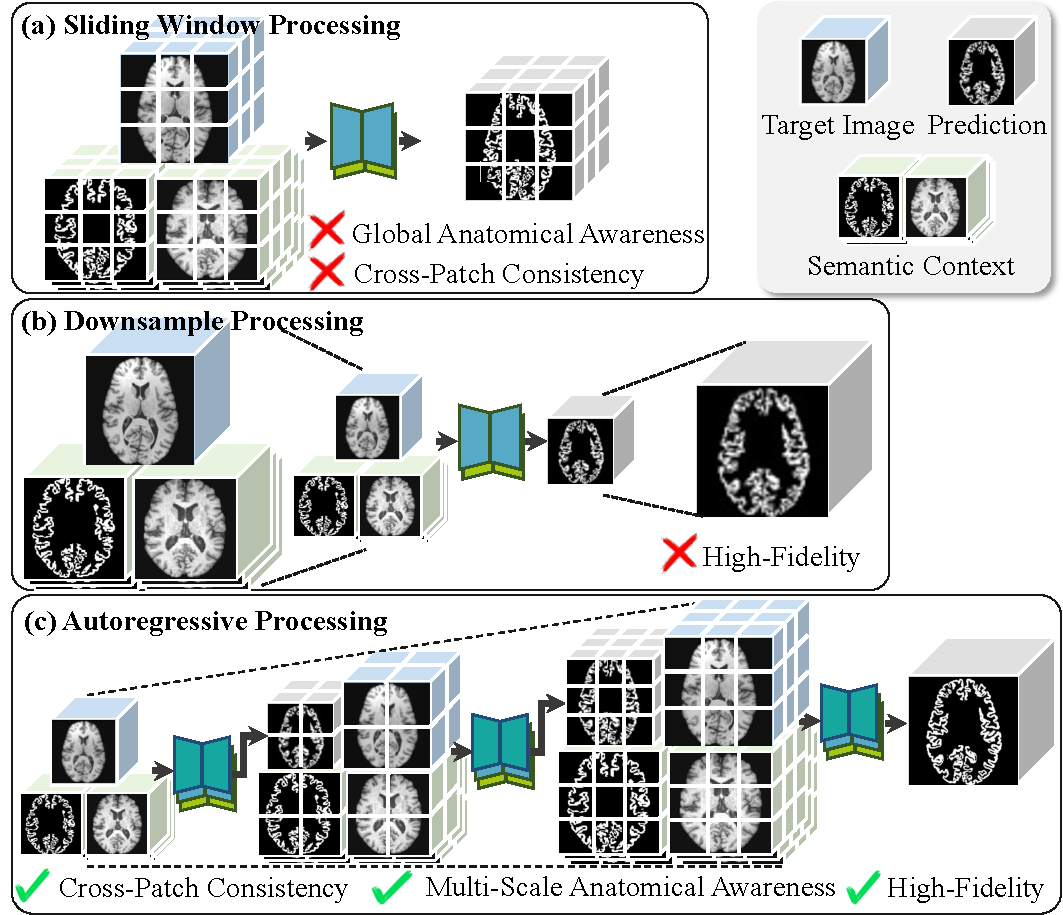
\includegraphics[width=0.472\textwidth]{intro_3.pdf}
\caption{
Illustration of different strategies for processing 3D medical images using ICL models. Due to the high resolution of volumetric data, direct end-to-end processing is often infeasible. The proposed next-scale autoregressive ICL framework progressively refines predictions from coarse to fine, producing full-resolution outputs.
}
\label{fig:intro_nsa}
\end{figure}


SegGPT~\cite{wang2023seggpt} and Painter~\cite{wang2023images} have demonstrated the effectiveness of ICL in natural image domains. However, their performance is suboptimal when applied to medical images~\cite{hu2025building}. Models such as UniverSeg~\cite{butoi2023universeg} and One-Prompt~\cite{wu2024one}, trained on medical imaging data, have shown promising results on 2D medical image segmentation tasks. Neuralizer~\cite{czolbe2023neuralizer} further extends ICL to a wider range of 2D tasks, including denoising and skull stripping. However, when applied to 3D data, they suffer from the loss of topological correlations and volumetric context. More recently, Neuroverse3D~\cite{hu2025building} has extended ICL to 3D neuroimaging by introducing adaptive context processing and architectural designs addressing the computational challenges of volumetric data. 

However, a major challenge is that current models remain constrained to operate at predetermined low spatial resolutions, which restricts their ability to capture fine-grained anatomical details and preserve the fidelity of output images. Attempts to increase output resolution via sliding-window strategies face the challenge of disrupting the anatomical continuity of context and target images, which impairs accurate understanding and the transmission of task-specific guidance from the context. This creates a dilemma for the development and practical use of ICL models in medical imaging. Another pressing issue is the absence of a unified 3D ICL model in medical imaging that is jointly trained across multiple organs and diverse types of image processing tasks, leaving the full potential of ICL in this domain underexplored.

To overcome the aforementioned issues, we present Medverse, a universal 3D medical image model trained on a diverse collection of datasets spanning multiple organs, imaging modalities, clinical centers, and task types, including universal segmentation, transformation, and enhancement. We introduce a \textbf{Next-Scale Autoregressive ICL framework (NA-ICL)} that adopts a coarse-to-fine prediction strategy and supports arbitrary input resolutions (Figure~\ref{fig:intro_nsa}). By integrating multi-scale anatomical cues from both context and target images, NA-ICL effectively balances global semantics with local details, improving prediction accuracy and producing consistent, full-resolution outputs while mitigating sliding-window artifacts. To enhance context perception under complex real-world conditions, we introduce a \textbf{Blockwise Cross-Attention Module (BAM)}, which enables long-range context-target interactions and alleviates spatial misalignment, while preserving computational and memory efficiency through spatial sparsity.


Our contributions are summarized as follows:
\begin{itemize}
    \item We introduce NA-ICL, a next-scale autoregressive in-context learning framework that enables the model to perform coarse-to-fine prediction. This allows the model to leverage global semantics and local details, producing high-fidelity and spatially consistent, full-resolution outputs.
    \item We introduce BAM, which enables long-range context-target interactions while maintaining minimal memory and computational overhead through spatial sparsity.
    \item Trained on a diverse collection of datasets, Medverse is extensively evaluated on held-out data spanning unseen centers, organs, species, and modalities. It achieves strong generalization and consistently outperforms existing in-context learning baselines across segmentation, transformation, and enhancement tasks.
\end{itemize}




% However, developing robust and generalizable models for diverse medical imaging tasks remains a significant challenge. Conventional models are often designed for specific tasks (e.g., liver segmentation, brain tumor detection) and trained on limited datasets with homogeneous characteristics. As a result, these models typically suffer from performance degradation when applied to unseen domains, such as new imaging modalities, institutions, or anatomical targets. The heterogeneity of clinical data—including differences in resolution, acquisition protocols, and anatomical focus—poses serious obstacles to the scalability and practicality of task-specific deep learning models. 




% 也有一些对于image transformation的universal model比如。。。。。这里要调研一下对比哪些。


% \subsection{3D Vision Models in Medical Imaging}


% \subsection{Cross-Attention and Multi-Context Feature Fusion}
